\section{Rate model}

\begin{frame}[c]{Rate model for VET}
  \begin{center}
    How can the vibrational energy transport be expressed in a simple model?
  \end{center}
\end{frame}

\begin{frame}[t]{Ansatz}
  $\rightarrow$ transition rate model for residues
  \begin{block}{Master equation}
    Change in energy of residue $i$
    $$ \frac{dE_i}{dt} = \sum_j \left( k_{ji} E_j - k_{ij} E_i \right) - k_{i,S} E_i + k_{S,i} E_S,$$
    with
    \begin{align*}
      k_{ij}& \qquad \text{transition rate from residue $i$ to residue $j$}\\
      k_{i,S}& \qquad \text{cooling rate from protein to solvent}\\
      k_{S,i}& \qquad \text{back rate from solvent to protein}
    \end{align*}

  \end{block}
\end{frame}

\begin{frame}[t, shrink=20]{Scaling rules}
  $\rightarrow$ diffusion model and detailed balance condition for transition rates
 \begin{block}{Backbone rates}
   $$k_{ij}^B = \frac{D_B}{\langle\Delta x_{ij}\rangle^2}  \sqrt{ \frac{f_j}{f_i} } $$ 
 \end{block} 

 \begin{block}{Polar contact rates}
   $$ k_{ij}^C = \frac{D_C}{\langle\Delta x_{ij} ^2\rangle} \sqrt{\frac{f_j}{f_i}}  $$
 \end{block}
 With
  \begin{align*}
    f& \qquad \text{degrees of freedom}\\
    \Delta x& \qquad \text{distance between closest atoms}
  \end{align*}

\end{frame}

\begin{frame}[c]{Rate model for VET}
  \begin{center}
    Can we apply the model, including the diffusion constants, globally if T is constant?
  \end{center}
\end{frame}

\begin{frame}[t]{Transition rates}
  \begin{columns}
    \begin{column}{0.5\textwidth}
      \begin{itemize}
        \item Polar + backbone rates 
      \end{itemize}
      \begin{center}
        \includegraphics[width=\linewidth]{total_rates_matrix.pdf}
      \end{center}
    \end{column}
    \begin{column}{0.5\textwidth}
      \includegraphics[width=\linewidth]{WW_snapshot1.png}  
    \end{column}
  \end{columns}

\end{frame}

\begin{frame}[t]{MEQ Results - Heater}
  \begin{center}
    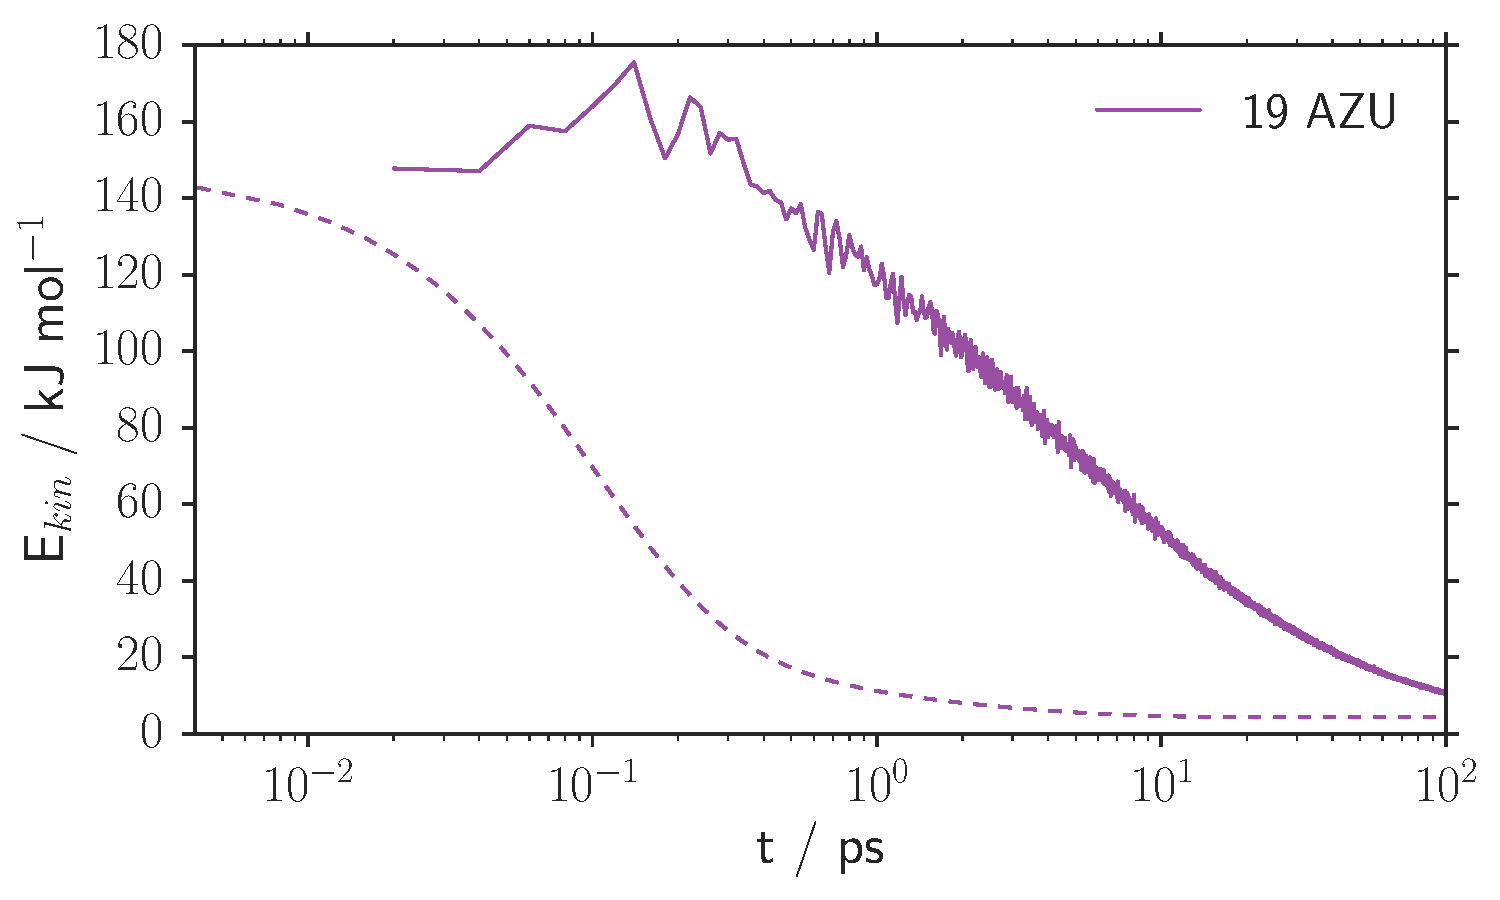
\includegraphics[width=0.8\linewidth]{E_kin_MEQ_MD_19AZU.pdf}
  \end{center}  
  $\rightarrow$ excited limbo state 19*?
\end{frame}

\begin{frame}[t]{MEQ Results - Neighbours}
  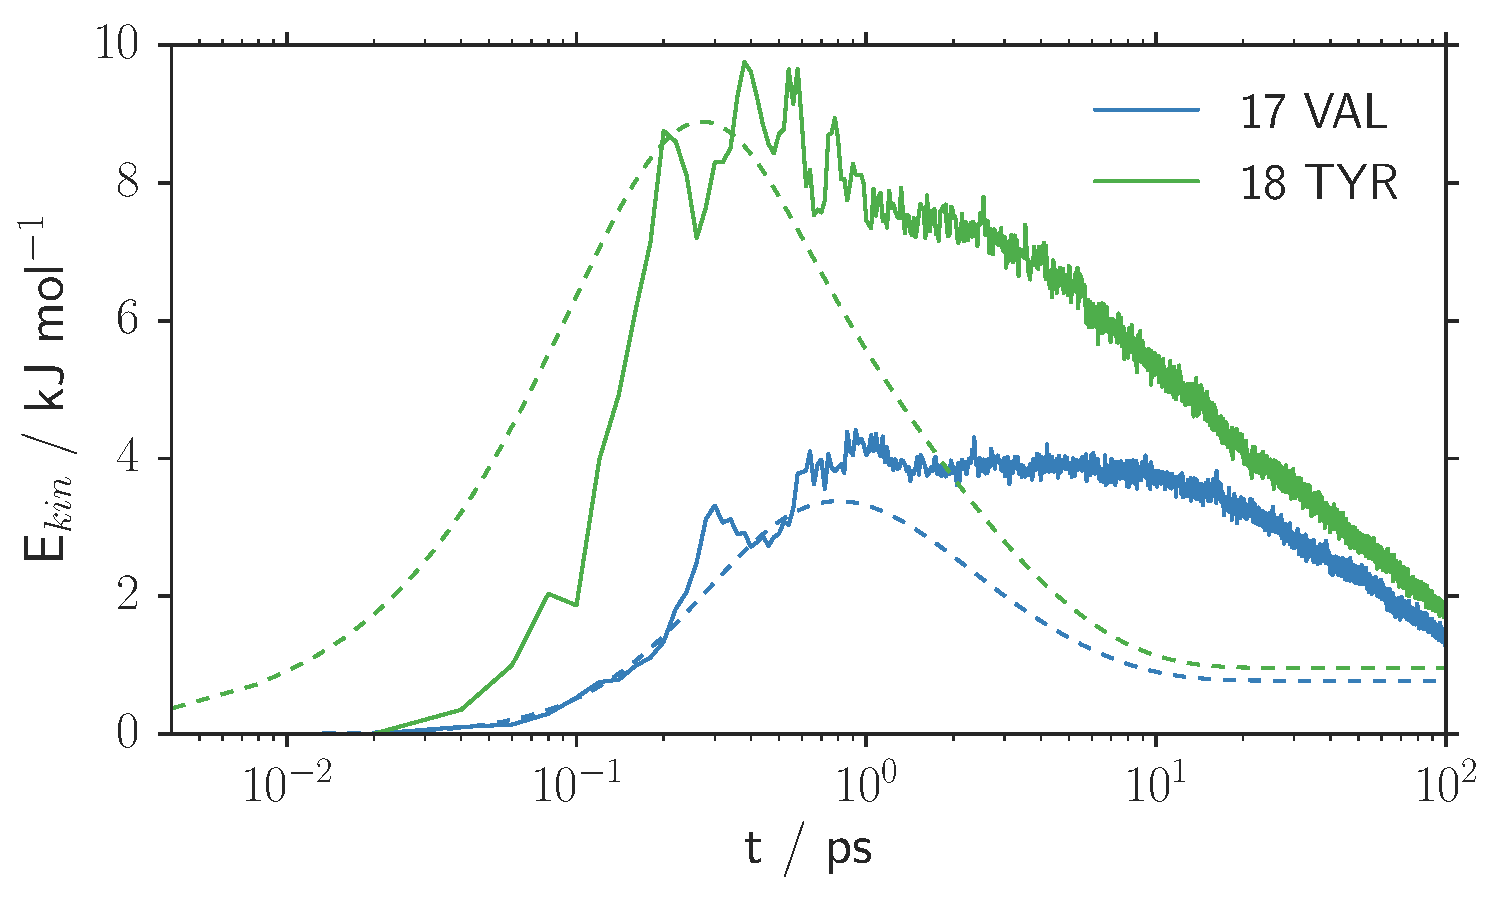
\includegraphics[width=0.7\linewidth]{E_kin_MEQ_MD_17VAL_18TYR.pdf}
  \begin{textblock*}{0.4\textwidth}(75mm,-8mm)
    \includegraphics[width=\linewidth]{WW_17_18.png}
  \end{textblock*}
  $\rightarrow$ shoulder to the right?
\end{frame}

\begin{frame}[t]{MEQ Results - Polar contacts}
  \includegraphics[width=0.7\linewidth]{E_kin_MEQ_MD_7GLU_8AHA_9ARG.pdf}
  \begin{textblock*}{0.4\textwidth}(75mm,-8mm)
    \includegraphics[width=\linewidth]{WW_7_8_9.png}
  \end{textblock*}
  $\rightarrow$ overestimation of $D_C$?
\end{frame}
